\documentclass[11pt,a4paper]{article}

%
% Packages
%
\usepackage[T1]{fontenc} % Output font encoding for international characters
\usepackage[utf8]{inputenc} % Required for inputting international characters
\usepackage{amsmath,amsthm,amssymb}
\usepackage[svgnames]{xcolor}
\usepackage[english,french]{babel}
\usepackage{multicol}
\usepackage{pstricks,pst-node,pst-text,pst-poly,pst-3d}
\usepackage{enumitem}
\usepackage{sidenotes}
\usepackage{graphicx} % Required to insert images
\usepackage{array}
\usepackage{booktabs} % Required for better horizontal rules in tables
\usepackage{titlesec} % Required for modifying sections
\usepackage{tikz}
\usetikzlibrary{trees}
\usepackage{verbatim}

%
% Constant and Variables
%
\setlength{\textwidth}{175mm}
\setlength{\textheight}{255mm}
\setlength{\oddsidemargin}{-10mm}
\setlength{\topmargin}{-15mm}
\setlength{\parskip}{0.2cm}
\definecolor{vertfonce}{rgb}{0,0.5,0}
% Set the overall layout of the tree
\tikzstyle{level 1}=[level distance=3.5cm, sibling distance=3.5cm]
\tikzstyle{level 2}=[level distance=3.5cm, sibling distance=2cm]
% Define styles for bags and leafs
\tikzstyle{bag} = [text width=4em, text centered]
\tikzstyle{end} = [circle, minimum width=3pt,fill, inner sep=0pt]

%
% Custom commands
%

\newcommand{\ds}{\displaystyle}
\newcommand{\scr}{\scriptscriptstyle}
\newcommand{\bs}[1]{\ensuremath{\boldsymbol{#1}}}

%
% Header
%
\newcommand{\header}[2]{

\noindent {\sc HEIG--VD} \hfill Probabilités et Statistique\newline 
\noindent {Corrigé Etudiant} \hfill 2021-2022\newline
\hrule
\vspace{3mm}
\noindent {\bf Thème : #1} \hfill Solution de la #2
\vspace{5mm}
\hrule
\vspace{7mm}
}
%

%
\newcommand{\separation}{{\begin{center}\rule{10cm}{0.25pt}\end{center}}\noindent} % crée une barre
%

%
% Math
%
\newcommand{\Real}{\mathbb R}
\newcommand{\RPlus}{\Real^{+}}
\newcommand{\norm}[1]{\left\Vert#1\right\Vert}
\newcommand{\abs}[1]{\left\vert#1\right\vert}
\newcommand{\setn}[1]{\left\{#1\right\}_{\scriptscriptstyle n \ge 1}}
\newcommand{\set}[1]{\left\{#1\right\}}
\newcommand{\seq}[1]{\left<#1\right>}
\newcommand{\eps}{\varepsilon}
\newcommand{\To}{\longrightarrow}
\newcommand{\Prob}{\rm{P}}
\newcommand{\F}{\mathcal{F}}
\newcommand{\h}{\mathcal{H}}
\newcommand{\M}{\mathcal{M}}
\newcommand{\X}{\mathcal{X}}
\newcommand{\N}{\mathcal{N}}
\newcommand{\E}{{\rm E}}
\newcommand{\Hnull}{{\rm H}_{0}}
\newcommand{\Hone}{{\rm H}_{1}}
\newcommand{\Var}{{\rm Var}}
\newcommand{\Cov}{{\rm Cov}}
\newcommand{\sign}{{\rm sign}}
\newcommand{\med}{{\rm med}}
\newcommand{\tr}{{\rm tr}}
\newcommand{\T}{{\text{\tiny \rm T}}}
\newcommand{\minf}{- \, \infty}
\newcommand{\intervalle}[4]{\mathopen{#1}#2\mathpunct{},#3\mathclose{#4}}
\newcommand{\intervalleff}[2]{\intervalle{[}{#1}{#2}{]}}
\newcommand{\intervalleof}[2]{\intervalle{]}{#1}{#2}{]}}
\newcommand{\intervallefo}[2]{\intervalle{[}{#1}{#2}{[}}
\newcommand{\intervalleoo}[2]{\intervalle{]}{#1}{#2}{[}}
\newcommand*\conj[1]{\overline{#1}}
\newcommand*\mean[1]{\overline{#1}} 

%
% Section
%
\titleformat
{\section} % Section type being modified
[block] % Shape type, can be: hang, block, display, runin, leftmargin, rightmargin, drop, wrap, frame
{\Large\bfseries} % Format of the whole section
{\assignmentQuestionName~\thesection} % Format of the section label
{6pt} % Space between the title and label
{} % Code before the label
\titlespacing{\section}{0pt}{0.5\baselineskip}{0.5\baselineskip} % Spacing around section titles, the order is: left, before and after

%
% Subsection
%
\titleformat
{\subsection} % Section type being modified
[block] % Shape type, can be: hang, block, display, runin, leftmargin, rightmargin, drop, wrap, frame
{} % Format of the whole section
{\alph{subsection})} % Format of the section label
{4pt} % Space between the title and label
{} % Code before the label
\titlespacing{\subsection}{0pt}{0.5\baselineskip}{0.5\baselineskip} % Spacing around section titles, the order is: left, before and after


%
%	Custom Exercice Environnment
%------------------------------------------------
\newcommand{\assignmentQuestionName}{Exercice} % The word to be used as a prefix to question numbers

% Environment to be used for each question in the assignment
\newenvironment{exo}{
	\vspace{0.5\baselineskip} % Whitespace before the question
	\section{} % Blank section title (e.g. just Exercice 2)
}

% Command to print a question sentence
\newcommand{\donnee}[1]{
	\noindent{Donnée: }
	\emph{#1}
	\vspace{0.5\baselineskip} % Whitespace afterwards
}

% Environment for subexercice, takes 1 argument - the name of the section
\newenvironment{subexo}[1]{
	\subsection{\itshape{#1}}
}

% Command to print a box that breaks across pages with the question answer
\newcommand{\answer}[1]{#1}
%------------------------------------------------

\frenchspacing


\begin{document}
	\header{probabilités conditionnelles et indépendance}{Série 2}
	%
	% Exercice 1
	%
	\begin{exo}
  \donnee{Une petite chenille descend doucement, lentement le long du grillage représenté dans la Figure 1. À chaque point gras de la figure appelé épissure, elle choisit la maille à votre gauche une fois sur trois, la maille à votre droite deux fois sur trois. La chenille descend quatre niveaux.}
  \begin{subexo}{Déterminer la loi de probabilité de X i.e. les probabilités $P(X = x)$ avec $x = 0, 1, 2, 3, 4$.}
    \begin{center}
    \end{center}
  \end{subexo}
	\begin{subexo}{De quelle distribution est issue la variable aléatoire X ? Préciser ses paramètres.}´
	\end{subexo}

\end{exo}


	%
	% Exercice 2
	%
	\begin{exo}
  \donnee{Sur le chemin de l’école, un étudiant de la HEIG–VD s’arrête toujours à la même station-service pour faire le plein d’essence. Il a constaté que les deux pompes de la station notées A et B ont la même probabilité d’être occupées. De plus, la probabilité que l’une des deux pompes au moins soit utilisée vaut 0.9 et celle que toutes les deux soient simultanément occupées est 0.5.}

  Pour faciliter la compréhension de cet exercice, on peut réaliser un diagramme de Venn.
  \begin{center}\includegraphics[scale=0.5]{ex2-diagrammeVenn}\end{center}
  Premièrement, posons que :
  \begin{multicols}{4}
    \begin{enumerate}[label=\alph*), parsep=0cm, itemsep=3mm, topsep=3mm]
      \item[ ] AO = La pompe A est occupée
      \item[ ] AL = La pompe A est libre
      \item[ ] BO = La pompe B est occupée
      \item[ ] BL = La pompe B est libre
    \end{enumerate}
  \end{multicols}
  \begin{center}$\Omega = \{(AL,BL),(AO,BL),(AL,BO),(AO,BO)\}$ \text{, évènements pas équiprobable !!!}\end{center}
  On sait que les probabilités que A soit libre sont les mêmes pour B. On note :
  \begin{center}$P(\{AL\}) = P(\{BL\})$\end{center}
  On sait aussi que :
  \begin{enumerate}
    \item[ ] $P(\text{au moins une pompe soite occupée}) = 0.9$
    \item[ ] $P(\text{les deux pompes soient occupées}) = 0.5$
    \item[ ] $P(\Omega) = 1$
  \end{enumerate}
  \begin{subexo}{Calculer la probabilité que les deux pompes soient disponibles.}
    Parmis les évènements probables on sait que :
    \begin{center}$P\{(AO,BL),(AL,BO),(AO,BO)\} = 0.9$\end{center}
    Puisque nous cherchons la probabilité du couple manquant $(P\{(AL,BL)\})$, on pose :
    \begin{center}$P(\Omega) = P\{(AL,BL)\} + P\{(AO,BL),(AL,BO),(AO,BO)\}$\end{center}
    En remplaçant les probabilités connues par leurs valeurs, on obtient :
    \begin{center}$1 = P\{(AL,BL)\} + 0.9$\end{center}
    On peut donc en conclure que $P\{(AL,BL)\}  = 0.1$ et donc que la probabilité que la pompe A et B soient libre est de $0.1$
  \end{subexo}
\begin{subexo}{Déterminer la probabilité que la pompe A soit libre.}
  Rappel : $P(A\cup B) = P(A) + P(B) - P(A \cap B)$ \\ \\
  Premièrement, on pose la formule énoncée dans le rappel en remplaçant avec nos valeurs :
  \begin{center}$P(AL\cup BL) = P(AL) + P(BL) - P(AL \cap BL)$\end{center}
  Maintenant, essayons d'exprimer $P(AL\cup BL)$ avec ce que nous connaissons : \\
  Avec la Loi de De Morgan on a :
  \begin{center}$P(\overline{AL\cup BL}) = P(\overline{AL} \cap \overline{BL}) = P(AO \cap BO)$\end{center}
  On sait que $P\{(AO,BO)\}=0.5$ donc que $P(AO \cap BO)=0.5$, on peut donc poser :
  \begin{center}$P(\overline{AL\cup BL}) = 1 - P(AL \cup BL)$\end{center}
  À présent on sait que :
  \begin{enumerate}
    \item[ ] $P(AL \cup BL) = 0.5$
    \item[ ] $P(AL \cap BL) = 0.1$ , voir exercice $a)$
  \end{enumerate}
  On peut donc compléter la formule $P(AL\cup BL) = P(AL) + P(BL) - P(AL \cap BL)$ avec les valeurs :
  \begin{center}
    $0.5 = P(AL) + P(BL) - 0.1$
  \end{center}
  Comme ennoncé en début d'exercice, on a $P(AL) = P(BL)$. On peut donc poser :
  \begin{center}
    $2P(AL) = 0.6$ \\ $P(AL) = 0.3$
  \end{center}
  On peut donc conclure que les probabilités que la pompe A soie libre sont de 0.3
\end{subexo}
\begin{subexo}{Calculer la probabilité que la pompe A soit occupée mais la pompe B disponible}
  Posons simplement la somme des probabilités que A soit occupée
  \begin{center}
    $P(AO) = P(AO \cap AO) + P(AO \cap BL)$
  \end{center}
  Sachant que $P(AL) = 0.3$ , on déduit que $P(AO) = 0.7$. On peut donc retourner la formule au-dessus pour obtenir :
  \begin{center}
    $P(AO \cap BL) = P(AO) - P(AO \cap AO)$
  \end{center}
En remplaçant par les valeurs connues on a :
\begin{center}
  $P(AO \cap BL) = 0.7 - 0.5 = 0.2$
\end{center}
On peut donc dire que la probabilité que la pompe A soit occupée et que la pompe B disponible est de $0.2$
\end{subexo}
\end{exo}


	%
	% Exercice 3
	%
	\begin{exo}
  \donnee{Une platforme petrolière a été construite à une hauteur de 8 mètres au 
  dessus du niveau
  de la mer. Selon les statistiques, les vagues atteignent le plateau de la plate-forme 
  une année donnée avec probabilité 0.05. On admet que les vagues parviennent au plateau 
  indépendamment des années}
  \begin{subexo}{Déterminer la probabilité qu'a partir de cette année les vagues 
    déferleront sur la plate-forme pour la première fois dans l'une des 
    cinq prochaines années}
    On se rappelle la théorie sur la loie géométrique et on se rappelle qu'elle compte le nombre
    d'essaie necessaire avant d'avoir la première épreuve réussite.
    Nous avons comme dans l'exercice précédent une suite d'épreuve indépendante avec une probabilité
    1-p d'échouée. Définission p la probabilité que les vagues atteignent la platforme.
    nous avons la probabilité que "les vagues atteignent la platforme dans les 5 prochaines années"
    qui est égale à la proba qu'elle les atteignent l'année prochaine, ou qu'elle ne réussisent pas la première année, 
    mais y arrivent l'année suivante, ou durant la troisième année(mais pas durant les deux premières)
    etc.
    Donc la proba vaut 
    \[
    0.05^1 + 0.95\cdot0.05 + 0.95^2\cdot0.05  + 0.95^3\cdot0.05  + 0.95^4\cdot0.05  
    \]
    Donc la proba = 0.226219
  \end{subexo}
  \begin{subexo}{En sachant que les vavues ne parviendront pas au plateau au minimum pendant les 
    cinq prochaines années, cacluler la probabilité qu'elles déferleront sur la platforme pour la première fois exactement dans huit ans}
    Les vagues n'ont pas de mémoire, donc la proba ne change pas en sachant que les 5 prochaines années les vagues ne dépasseront pas le niveau.
    Ca revient à calculer la proba que durant les 3 prochaines années les vagues ne dépasseront pas le niveau
    \[0.95^2 \cdot 0.05 = 0.045125\]
    
  \end{subexo}
\end{exo}

	%
	% Exercice 4
	%
	\begin{exo}
  \donnee{Pour modéliser le maximum annuel des débits d'une certaine rivière, les hydrologues utilisent habituellement une variable aléatoire X issue d'une distribution de Gumbel dont la fonction de répartition est donnée par: $F_x(x) = e^{-e^{-\frac{x-a}{b}}}´$ où $x \in \Real$. À partir des maxima annuels des débits relevés de 1971 à 1995 à une station située sur la rivière, les paramètres a et b ont été estimés $25.5$ et $7.98$ respectivement.}
	\begin{subexo}{Calculez la probabilité qu'une année donnée le maximum des débits soit supérieur à $35.5$  $m^3/s$}
  		\begin{center}
  			La fonction de répartition étant déjà donnée avec a et b,
  		\end{center}
		\begin{align*}
			P(X > 35.5) &= 1 - P(X \leq 35.5) \\
			&= 1 - F_x(35.5) \\
	  		&= 1 - e^{-e^{-\frac{x-7.98}{25.5}}}\\
	  		&\approx 0.248
	 	\end{align*}
  	\end{subexo}
  	\begin{subexo}{La période de retour T caractérise la durée moyenne s'écoulant entre deux occurences consécutives d'un même événement. Plus précisément, elle est définie par $ T = \dfrac{1}{1- F_x(x)}$. Calculez le débit maximal annuel x correspondant à une période de retour de 100 ans. Ce débit est interprété comme étant le débit maximal annuel qui sera dépassé en moyenne une fois tous les 100 ans.}
	\begin{center}
		On cherche à calculer T = 100
	\end{center}
	\begin{align*}
		100 &=  \dfrac{1}{1- F_x(x)}\\
		0.99 &= F_x(x) \\
		0.99 &= e^{-e^{-\frac{x-a}{b}}} \\
		-\ln(0.99) &= e^{-\frac{x-a}{b}} \\ 
		\ln{-\ln(0.99)} &= -\frac{x-a}{b} \\ 
		b\cdot \ln{-\ln(0.99)} &= a-x \\ 
		x &= a-b\cdot \ln{-\ln(0.99)} \\ 
		&= 25.5 -7.98\cdot \ln{-\ln(0.99)} \\
		&\approx 62.21
	\end{align*}
	\end{subexo}
\end{exo}


	%
	% Exercice 5
	%
	\begin{exo}
  \donnee{Considérons deux variables aléatoires X et Y dont les histogrammes se trouvent dans la figure ci-dessous.\\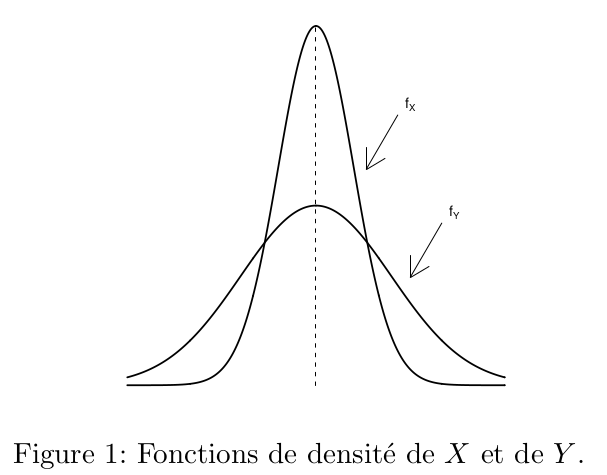
\includegraphics[width=8cm]{ex5.png}
  \\En n’effectuant aucun calcul, l’écart-type de X est-il plus grand que celui de Y ?
  }
  L'écart type est plus grand dans la figure x car les données sont plus écartées que dans la figure y
\end{exo}


	%
	% Exercice 6
	%
	\begin{exo}
  \donnee{La société Gloup s’intéresse à la capacité de détection que possède le filtre bayesien anti-spam qu’elle vient d’installer. Dans la liste des mots et symboles permettant de détecter des messages publicitaires figurent les mots “viagra” et “miracle”. Par simplification, notons ces mots 1 et 2 et les probabilités:
    \\\indent$P_i$ : probabilité qu’un mot choisi au hasard dans un message électronique est le mot i en sachant que le message est un spam
    \\\indent$Q_i$ : probabilité qu'un mot choisi au hasard dans un message électronique est le mot i en sachant que le message n’est pas un spam
    \\valent respectivement $P_1$ = 0.05, $P_2$ = 0.1 et $Q_1$ = 0.001, $Q_2$ = 0.5. Supposons que dans chaque type de messages électroniques, les mots de la liste se trouvent indépendamment les uns des autres dans les messages. La proportion de messages spam reçus par la société Gloup vaut 0.9. En sachant que les mots “viagra” et “miracle” figurent tous les deux une fois dans le même message électronique, déterminer la probabilité qu’il s’agisse d’un spam.}
  \begin{flushleft}
    Soit l'évènement aléatoire $S$ = "le message est un spam".
    Avec la donnée nous avons:
    \\Mot1 = "Viagra" avec $P_1 =P(M_1|S)= 0.05$ et $Q_1=P(M_1|\conj{S})=0.001$
    \\Mot2 = "Miracle" avec $P_2=P(M_2|S)= 0.1$ et $Q_2=P(M_2|\conj{S})=0.5$
    \\$P(S) = 0.9$ et $P(\conj{S}) = 0.1$
    \\La probabilité cherchée est $P(S|M_1 \cap M_2)$ qui peut s'obtenir avec la formule de bayes totale:
    \\ $P(S|M_1 \cap M_2) = \dfrac{P(M_1 \cap M_2|S)\cdot P(S)}{P(M_1 \cap M_2)}$
    \\ avec $P(M_1 \cap M_2)$
    \\ $=P(M_1 \cap M_2 | S) \cdot P(S) + P(M_1 \cap M_2 | \conj{S})\cdot P(\conj{S})$
    \\ $=P(M_1|S)\cdot P(M_2|S) \cdot P(S) + P(M_1| \conj{S}) \cdot P(M_2 | \conj{S})  \cdot  P(\conj{S})$
    \\ $= P_1P_2 \cdot P(S) + Q_1Q_2\cdot P(\conj{S})$
    \\ Numériquement,
    \\ $P(M_1 \cap M_2) = P_1P_2 \cdot P(S) + Q_1Q_2\cdot P(\conj{S}) = 0.05\cdot 0.1 \cdot 0.9 + 0.001\cdot 0.5 \cdot 0.1 = 0.00455$
    \\ $P(M_1\cap M_2|S)\cdot P(S) = P_1P_2 \cdot P(S) = 0.05 \cdot 0.1 \cdot 0.9 = 0.0045$
    \\ Donc
    \\  $\dfrac{P(M_1|S)\cdot P(S)}{P(M_1)} = \dfrac{0.0045}{0.00455} = 0.989$
  \end{flushleft}
\end{exo}


	%
	% Exercice 7
	%
	\begin{exo}
  \donnee{En sachant que pour le jour de la rentrée académique, la météo avait annoncé de la pluie le matin alors que le comportement de la grenouille avait laissé présager du soleil, calculer la probabilité qu'il allait faire beau à Yverdon le matin de la rentrée.}
 \begin{flushleft}
 	L'exercice demande de prédire $P(E | \conj{F} \cap G)$. C'est à dire qu'il fasse beau $E$ sachant que la météo prédit la pluie $\conj{F}$ et que la grenouille prédise le beau temps $G$.
  \end{flushleft}
  \begin{align*}
  	P(E | \conj{F} \cap G) &= \dfrac{P(\conj{F} \cap G |E)\cdot P(E)}{P(\conj{F} \cap G)}
  	\\&= \dfrac{P(\conj{F}|E)\cdot P(G|E)\cdot P(E)}{P(\conj{F} \cap G |E)\cdot P(E)+ P(\conj{F} \cap G |\conj{E})\cdot P(\conj{E})}
  	\\ &= \dfrac{0.7\cdot 0.02 \cdot 0.95}{0.7 \cdot 0.0019 + 0.3 \cdot 0.049}
  	\\ &=0.475
  \end{align*}
\end{exo}

	
	%3
	% Footer
	%
	\vfill
	\hrule
	\vspace{2mm}
	\noindent {\tiny Corrigé Etudiant - TIC} \hfill {\tt \tiny \today}
\end{document}
